\documentclass[10pt, conference, compsocconf]{IEEEtran}




%%% PAGE DIMENSIONS
%\usepackage{geometry} % to change the page dimensions
%\geometry{a4paper} % or letterpaper (US) or a5paper or....
% \geometry{margins=2in} % for example, change the margins to 2 inches all round
% \geometry{landscape} % set up the page for landscape
%   read geometry.pdf for detailed page layout information

\usepackage{graphicx} % support the \includegraphics command and options

% \usepackage[parfill]{parskip} % Activate to begin paragraphs with an empty line rather than an indent

%%% PACKAGES
\usepackage[utf8]{inputenc} % set input encoding (not needed with XeLaTeX)
\usepackage{listings}
\usepackage[scaled]{beramono}
\usepackage[T1]{fontenc}
\usepackage{xcolor}
\usepackage{booktabs} % for much better looking tables
\usepackage{array} % for better arrays (eg matrices) in maths
\usepackage{paralist} % very flexible & customisable lists (eg. enumerate/itemize, etc.)
\usepackage{verbatim} % adds environment for commenting out blocks of text & for better verbatim
\usepackage{subfig} % make it possible to include more than one captioned figure/table in a single float
% These packages are all incorporated in the memoir class to one degree or another...
\usepackage{algorithm}
\usepackage{algpseudocode}
\usepackage{amsmath}
\usepackage{amsthm}

%%% HEADERS & FOOTERS
\usepackage{fancyhdr} % This should be set AFTER setting up the page geometry
\pagestyle{fancy} % options: empty , plain , fancy
\renewcommand{\headrulewidth}{0pt} % customise the layout...
\lhead{}\chead{}\rhead{}
\lfoot{}\cfoot{\thepage}\rfoot{}

%%% SECTION TITLE APPEARANCE
%\usepackage{sectsty}
%\allsectionsfont{\sffamily\mdseries\upshape} % (See the fntguide.pdf for font help)
% (This matches ConTeXt defaults)

%%% ToC (table of contents) APPEARANCE
%\usepackage[nottoc,notlof,notlot]{tocbibind} % Put the bibliography in the ToC
%\usepackage[titles,subfigure]{tocloft} % Alter the style of the Table of Contents
%\renewcommand{\cftsecfont}{\rmfamily\mdseries\upshape}
%\renewcommand{\cftsecpagefont}{\rmfamily\mdseries\upshape} % No bold!

%%% END Article customizations

%%% The "real" document content comes below...

\title{MapReduce on a Chord Distributed Hash Table}
\author{\IEEEauthorblockN{Andrew Rosen \qquad Brendan Benshoof \qquad Matt Erwin \qquad Robert W. Harrison \qquad Anu G. Bourgeois}
\IEEEauthorblockA{Department of Computer Science\\
Georgia State University\\
Atlanta, Georgia\\
rosen@cs.gsu.edu}
}

%\author{
%Andrew Rosen \qquad Brendan Benshoof \qquad Matt Erwin \qquad Robert Harrison \qquad Anu Bourgeois  \\Department of Computer Science, Georgia State University\\ 34 Peachtree St NW \\ Atlanta, Georgia 30303\\  rosen@cs.gsu.edu }
%\date{} % Activate to display a given date or no date (if empty),
         % otherwise the current date is printed 


\hyphenation{op-tical net-works semi-conduc-tor Chord-Reduce Map-Reduce Data-Nodes Name-Nodes}

\begin{document}
\lstset{language=Python, basicstyle= \footnotesize\ttfamily ,showstringspaces=false, frame=single, commentstyle=\itshape\color{gray}, identifierstyle=\color{black},  keywordstyle=\bfseries\color{red!40!black}, stringstyle=\color{blue}} 
\maketitle

\begin{abstract}


This paper proposes ChordReduce, a novel implementation of Chord that acts as middleware for creating and running MapReduce jobs. ChordReduce satisfies the desired properties for a distributed MapReduce platform. Chord is a peer-to-peer networking protocol for distributed storage and file sharing that provides $\log_{2}(n)$ lookup time for any particular file or node.  Files and nodes are evenly distributed across a ring overlay and organized such that the responsibilities of a failed node are automatically reassigned.  ChordReduce leverages these features to distribute Map and Reduce tasks evenly among nodes and maintain a high degree of robustness during execution.  The loss of a single node or a group of nodes during execution does not impact the soundness of the results and their tasks are automatically reassigned.  An additional benefit is that nodes joining the ring during runtime can automatically have work distributed to them.

MapReduce frameworks are generally hierarchical, with the responsibility of scheduling work, distributing data and tasks, and tracking progress at the top.  This leads to centralized MapReduce implementations having a single point of failure.  A MapReduce framework with both responsibility and work distributed among its members would eliminate the need for a central source of coordination.  An ideal MapReduce framework would need to be highly scalable, fault-tolerant during execution, able to handle a high degree of churn, and minimize the amount of traffic that results from maintaining the network. 

Our experiments show that ChordReduce is an efficient implementation of MapReduce. The applications are far-reaching, especially for big data problems and those that are massively parallel. Implementing MapReduce on a Chord peer-to-peer network demonstrates that the Chord network is an excellent platform for distributed and concurrent programming in cloud and loosely coupled environments.

\end{abstract}


\begin{IEEEkeywords}
MapReduce; P2P; Parallel Processing; Peer-to-Peer Computing; Cloud Computing; Middleware;

\end{IEEEkeywords}


\textit{Italics in the text indicate that I want to express this idea but with different words or a reference.}
\section{Introduction}

\textit{The story we want to tell s that map redce is awesome.  Here is alist of pros for ma reduce. Awesome but designed for data center use, which is a subset of the possible configuration but really the only one explored in depth. Introduce single point of failure and if we want to explore using mapreduce in  a more generalized manner we have to solve the problem of a single point of failure.  P2P frameworks are explicitly designed to eliminate single points of failure, scale, wax platonic on virtues of P2P. 
We were motivated to look at it from a more abstract point of view and ask how can we do map reduce jobs over a more generalized/distributed configuration.  THis paper presents ChordReduce}



Google's MapReduce \cite{mapreduce} paradigm has rapidly become an integral part in the world of data processing and is capable of efficiently executing numerous Big Data programming and data-reduction tasks.  By using MapReduce, a user can take a large problem, split it into small, equivalent tasks and send those tasks to other processors for computation.  The results are sent back to the user and combined into one answer.  \textit{One of the reasons MapReduce has become so important is that many problems/tasks can be posed in the form of Map and Reduce tasks.} \footnote{The story we want to tell in this paragraph is that map reduce is awesome and why it is awesome.}

Many popular platforms for MapReduce, such as Hadoop \cite{Hadoop}, are designed with data centers in mind


% http://wiki.apache.org/hadoop/Virtual%20Hadoop  Hapdoop assumptions.
Many popular platforms for MapReduce, such as Hadoop \cite{Hadoop}, utilize a central source of coordination and organization to store and operate on data. The hierarchical structure of Hadoop results in a single point of failure at the node that concentrates the results and also requires a complicated scheme for handling node failures.

However, Hadoop and other MapReduce platforms are designed from the perspective of \textit{being used for high performance computing and data centers} and \textit{not in the context of P2P or volunteer computing}. These MapReduce platforms are highly centralized and tend to have single points of failure\footnote{reference of Hadoop single point of failure and schedulers goes here} as a result.   A centralized design assumes that the network is relatively unchanging and does not usually have mechanisms to hand node failure during execution or, conversely, cannot speed up the execution of a job by adding additional workers on the fly.   Finally, learning curve for deploying a system to perform MapReduce and develop programs to run on the \textit{is annoying}.  \footnote{Awesome but designed for data center use, which is a subset of the possible configuration but really the only one explored in depth. Introduce single point of failure and if we want to explore using mapreduce in  a more generalized manner we have to solve the problem of a single point of failure.}





%Suppose we have numerical calculation that we want to perform, such as calculating $\pi$.

Our paper presents our contributions:
\begin{itemize}
	\item We define the architecture and components of ChordReduce and demonstrate how they fit together to perform MapReduce jobs over a distributed system without the need of a central scheduler or coordinator, avoiding a central point of failure\footnote{TODO: defend why the starting node isn't considered to be this in corresponding section}. We also demonstrate how to create programs to solve MapReduce problems using ChordReduce (Section \textit{ChordReduceNum}). 
	\item We used Python to build a prototype system implementing ChordReduce and deployed it on Amazon's EC2. We created programs to solve Monte-Carlo computations and word frequency counts on our deployed network (Section \textit{ExperimentNum}).
	\item We prove that ChordReduce is scalable and highly fault tolerant, even under high levels of churn and can even benefit from churn under certain circumstances. Additionally, we show it is robust enough to reassign work during runtime in response to nodes entering and leaving the network (Section \textit{ResultsNum}).
	\item We contrast ChordReduce with similar architectures and identify future areas of fruitful research using ChordReduce (Section \textit{Future/Related  Work}). 





\end{itemize}
A note\footnote{I feel we have to justify why we want to use our system over stuff like Hadoop, either by showing distributed $>>$ centralized for MapReduce (not likely and would probably be seen as arrogant)  or defining use cases where we want or need a distributed system.}

%Chord \cite{Chord} is a peer-to-peer (P2P) protocol for file sharing and distributed storage that guarantees a high probability $\log_{2} n$ lookup time for a particular node or file in the network. It is highly fault-tolerant to node failures and churn, the constant joining and leaving of nodes.  It scales extremely well and the network requires little maintenance to handle individual nodes.  Files in the network are distributed evenly among its members.

%Our experiments demonstrate that the ChordReduce framework is highly scalable, solving problems significantly faster when distributed.  The larger the problem is, the greater the speedup gained by incorporating more nodes into the problem.  Our framework also provides a high level of robustness during execution;  we can lose many nodes to churn, and still process jobs successfully.  If we find a job requires more computational power, we can add more nodes to the job during runtime.

%While Chord could be used to implement a grid computing environment similar to BOINC \cite{boinc} or Folding@home \cite{folding}, it would be difficult to efficiently implement the MapReduce algorithm using grid computing tools. MapReduce uses persistent data to amortize the cost of distributing the data across the nodes over many calls, while grid environments typically transmit a transient bundle of data and computation to a volunteer node. BOINC and Folding@home use a master-slave architecture with a critical point of failure similar to Hadoop, while ChordReduce is a true peer-based approach.




\section{Background}
Chord and MapReduce are integral parts of ChordReduce.  We summarize these frameworks in this section.

\subsection{Chord}
Chord \cite{Chord} is a peer-to-peer (P2P) protocol for file sharing and distributed storage that guarantees a high probability $\log_{2} N$ lookup time for a particular node or file in the network. It is highly fault-tolerant to node failures and churn, the constant joining and leaving of nodes.  It scales extremely well and the network requires little maintenance to handle individual nodes.  Files in the network are distributed evenly among its members\footnote{This entire paragraph can probably be chopped up}.

As a distributed hash table (DHT), each member of the network and the data stored on the network is mapped to a unique $m$-bit key or ID, corresponding to one of  $2^m$ locations on a ring. 
The ID of a node and the node itself are referred to interchangeably.

In a traditional Chord network, all messages travel in one direction - upstream, hopping from one node to another with a greater ID until it wraps around.
A node in the network is responsible for all the data with keys \textit{above or upstream} his predecessor, up through and including its own ID.  If a node is responsible for some key, it is referred to being the successor of that key.

Robustness in the network is \textit{achieved} by having nodes backup their contents to their $s$ (often 1) immediate successors, the closest nodes upstream.  
This is done because when a node leaves the or fail, the most immediate successor would be responsible for the content its content.

\textit{To achieve scalability} nodes maintains a table of $m$ shortcuts, called the finger table, to other peers.   The $i$th entry of a node $n$'s finger table corresponds to the node that is the successor of the key $n+2^{i-1} \mod 2^m $.  Nodes route messages to the finger that is closest to the sought key without going past it, until it is received by the responsible node.  This provides Chord $\log_2(N)$ lookup time for any key \cite{Chord}.

Full details on how Chord handles nodes entering the network and leaving the network, as well the maintenance cycle, are beyond the scope of this paper and can be found \textit{references, plural} \cite{Chord}.

\begin{figure}
    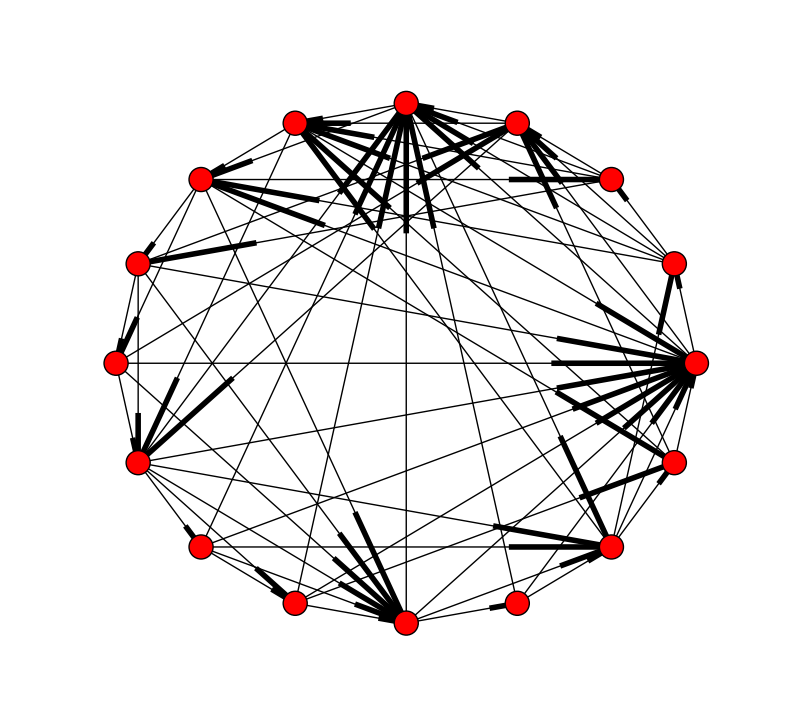
\includegraphics[width=\linewidth]{chordreal}
    \caption{A Chord ring 16 nodes where $m=4$.  The bold lines are incoming edges.  Each node has a connection to its successor, as well as 4 fingers, some of which are duplicates.}
    \label{chordreal}
\end{figure}





\subsection{MapReduce and Hadoop}
At its core, MapReduce \cite{mapreduce} is a system for division of labor, providing a layer of separation between the programmer and the more complicated parts of concurrent processing.  The programmer sends a large task to a master node, who then divides that task among slave nodes (which may further divide the task).  This task has two distinct parts: Map and Reduce.  Map performs some operation on a set of data and then produces a result for each Map operation.  The resulting data can then be reduced, combining these sets of results into a single set, which is further combined with other sets.  This process continues until one set of data remains.

The classic example given for MapReduce is counting the occurrence of each word in a collection of documents.  The master node splits up the documents into multiple blocks and sends them off to workers.  Each worker then goes through their blocks and creates a small word frequency list.  These lists are then used by other workers, who combine them into larger and larger lists, until the master node is left with a word frequency list of all the words in the documents. 



%The most popular platform for MapReduce is Hadoop \cite{Hadoop}. Hadoop is an open-source Java implementation deveolped by Apache and Yahoo! \cite{pavlo2009comparison}.  Hadoop has two components, the Hadoop Distributed File System (HDFS) and the Hadoop MapReduce Framework \cite{mrsurvey}.  Under HFDS, nodes are arranged in a heirarchical tree, with a master node, called the NameNode, at the top.  The NameNode is responsible for keeping track of which DataNodes posess which files as well as other metadata essential for controlling the netowork. MOVE THIS DOWN
 

One very popular open-source implementation of MapReduce is Apache's Hadoop \cite{Hadoop}.  Hadoop serves as both a distributed file system and framework for MapReduce \cite{shvachko2010hadoop}.  However,  Hadoop's MapReduce framework is very strongly tied to the Hadoop Distributed File System (HDFS) and the hierarchy of servers that is used by it.  Hadoop is centralized around the NameNode.  The NameNode's job is to organize and distribute information to the slave nodes, called DataNodes.  This makes the NameNode a single point of failure \cite{shvachko2010hadoop} in the network, as well as a potential bottleneck for the system \cite{hadoop-bottle}.

To do work on Hadoop, the user stores their data on the network.  This is handled by the NameNode, which equally apportions the data among the DataNodes.  When a user wants to run some analysis on the data or some subset the data, then that function is sent by the NameNode to each of the DataNodes that is responsible for the indicated data.   After the DataNode finishes processing, the result is handled by other nodes called Reducers which collect and reduce the results of multiple DataNodes.






\section{ChordReduce}
Marozzo et al. \cite{marozzo2012p2p} shows that adding additional fault-tolerance features to a MapReduce architecture is worth the added cost of maintenance, as the time lost due to node failures is greatly reduced.  However, Marozzo et al. do not explore the benefits of leveraging the properties of a P2P protocol to reduce the complexity of the architecture and completely distribute the responsibility of the task across the network.  As a result, P2P-MapReduce still relies on a ratio of masters to slaves to coordinate and organize the network, meaning a percentage of the network is unable to contribute processing power to the actual solving of a problem.   

Lee et al. \cite{leemap} explores the benefits of building a MapReduce module to run on top of Symphony \cite{symphony},  a P2P protocol.  Unlike Hadoop, this allows the MapReduce tasks to be executed without the need of a central source of coordination by distributing tasks over a bounded broadcast tree created at runtime.  The Symphony based MapReduce architecture would be greatly improved by the addition of components to handle the failure of nodes during execution.  As it stands now, if a node crashes the job will fail due to the loss of data.

While both of these papers have promising results and confirm the capability of our own framework, both solely look at P2P networks for the purpose of routing data and organizing the network. Neither examines using a P2P network as a means of efficiently distributing responsibility throughout the network and using existing features to add robustness to nodes working on Map and Reduce tasks.  

ChordReduce uses Chord to act as a completely distributed topology for MapReduce, negating the need to assign any explicit roles to nodes or have a scheduler or coordinator.  ChordReduce does not need to assign specific nodes the task of backing up work; nodes backup their tasks using the same process that would be used for any other data being sent around the ring.  Finally, results work their way back to a specified hash address, rather than a specific hash node, eliminating any single point of failure in the network.  These features help prevent a bottleneck from occurring. The result is a simple, distributed, and highly robust architecture for MapReduce.


\footnote{2/6/2014:  We could obtain data for jobs in one of two ways:  distribute at runtime (suitable for calculations) or store before hand and operate on them later(useful for actual data like wordcount)}

\subsection{Handling Node Failures in Chord}
Due to the potentially volatile nature of a peer-to-peer network, Chord has to be able to handle (or at the very least, tolerate) an arbitrary amount of churn.  Section II described how Chord gradually guides nodes into their correct locations after they join the network.  The same is true for when a node leaves the network; the stabilize procedure will guide nodes to their correct successors and predecessors.  However, we can exert more control over how to handle nodes leaving the network.

When a node $n$ changes his successor, $n$ asks if the successor is holding any data $n$ should be responsible for.  The successor looks at all the data $n$ is responsible for and sends it to $n$.  The successor does not have to delete this data. In fact, keeping this data as a backup is beneficial to the network as a whole, as $n$ could decide to leave the network at any point. 

Chord specifies two ways a node can leave the ring.  A node can either suddenly drop out of existence, or a node can tell the network he is about to leave, letting his successor and predecessor immediately perform the needed changes.

When a node politely quits, he informs both his successor and predecessor and gives them all the information they need to fill the resulting gap. He also sends all of the data he is responsible for to his successor, who becomes responsible for that data when the node leaves.  Fingers that pointed to that node would be corrected during the finger maintenance period.  This allows for the network to adjust to churn with a minimum of overhead.

It is unlikely that every time a node leaves the network, it will do so politely.  If a node suddenly quits, the data it had stored is lost. To prevent data from becoming irretrievable, a node periodically sends backups to its successor.  In order to prevent a cascade of backups of backups, the node only passes along what it considers itself responsible for.  What a node is responsible for changes as nodes enter and leave the network.  If a node's successor leaves, the node sends a backup to his new successor. 

Our prototype framework does not implement a polite disconnect;  when a node quits, it does so quickly and abruptly.  This design ensures that the  system would be able to handle churn under the worst of cases.  Polite quit could be implemented quite easily.


\textit{insert architecture layer diagram }  and \textit{insert work flow diagram.  Chord tree of stage, map , reduce.}

\subsection{Implementation}

\begin{figure}
    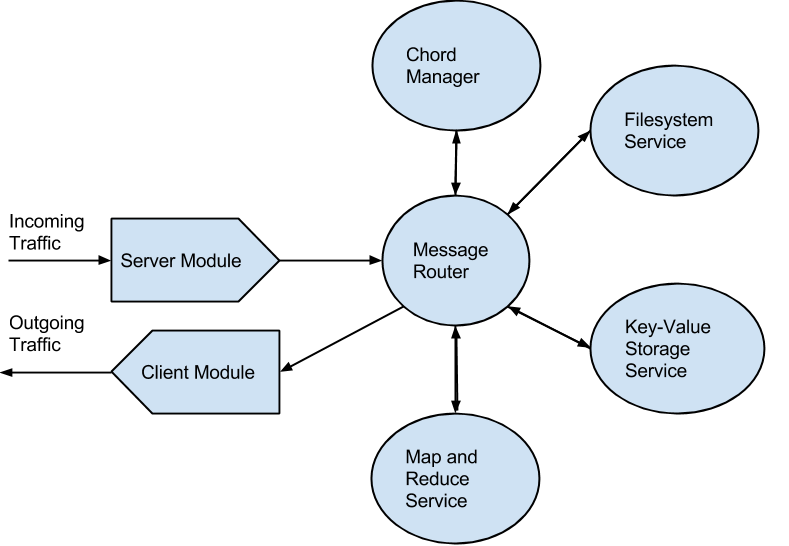
\includegraphics[width=\linewidth]{crArch}
    \caption{The basic architecture of a node in ChordReduce.  MapReduce runs as a service on top of each node.}
    \label{crArch}
\end{figure}

ChordReduce is a fully functional Chord implementation in Python.  Our installation was designed to be as simple as possible.  It consists of downloading our code \cite{code} and running chord.py.  A user can specify a port and IP of a node in the ring they wish to join.  The node will automatically integrate into the ring with this minimal information.  The ring as implemented is stable and well organized.  We created various services to run on top the network, such as a file system and distrubuted web server.  Our file system is capable of storing whole files or splitting the file up among multiple nodes the ring.  Our MapReduce module is a service that runs on top of our Chord implementation, similar to the file system (Fig. \ref{crArch}).  We avoided any complicated additions to the Chord architecture; instead we used the protocol's properties to create the features we desired in our MapReduce framework. 
  
In our implementation of MapReduce, each node takes on responsibilities of both a worker and master, much in the same way that a node in a P2P file-sharing service will act as both a client and a server.  Jobs still must start from a single location.  To start a job, the user contacts a node at a specified hash address and provides it with the tasks and data.  This address can be chosen arbitrarily or be a known node in the ring. The node at this hash address is designated as the stager.  

The job of this stager is to take the work and divide it into \emph{data atoms}, which are the smallest individual units that work can be done on.  This might be a line of text in a document, the result of a summation for a particular intermediate value, or a subset of items to be sorted.  The specifics of how to divide the work are defined by the user in a \emph{stage} function.  The data atoms are then each given a random hash and sent to the node responsible for that hash address, guaranteeing they are evenly distributed throughout the network.  The data atoms also contain the Map function and Reduce function as defined by the user.  A job ID is also included, so that data atoms from different jobs can be differentiated.  Once the data atoms are sent out, the stager's job is done and it behaves like any other node in the network. The staging period is the only time ChordReduce is vulnerable to churn, and only if the stager leaves the ring in the middle of sending out data atoms.  The user would get some results back, but only for the data the stager managed to send out.

Nodes that receive data atoms apply the Map function to the data to create result data atoms, which are then sent back to the stager's hash address (or some other user defined address).  This will take $\log_{2} n$ hops traveling over Chord's fingers.  At each hop, the node waits a predetermined minimal amount of time to accumulate additional results (In our experiments, this was 100 milliseconds).

Nodes that receive at least two results merge them using the Reduce function.  The results are continually merged until only one remains at the hash address of the stager. 

Once the reductions are finished, the user retrieves his results from the node at the stager's address.  This may not be the stager himself, as the stager may no longer be in the network.  The stager does not need to collect the results himself, since the work is sent to the stager's hash address, rather than the stager itself.  Thus, the stager could quit the network after staging, and both the user and the network would be unaffected by the change. % Here, we are leverging two features. First, we use the automatic assignment of responsibility to automatically route the data to the sucessor.  %Second, the same process Chord uses to backup files is used to backup the intermediate data. 

Similar precautions are taken for nodes working on Map and Reduce tasks.  Those tasks are backed up by a node's successor, who will run the task if the node leaves before finishing its work (e.g. the successor loses his predecessor).   The task is given a timeout by the node.  If the backup node detects that the responsible node has failed, he starts the work and backs up again to \emph{his} successor.  Otherwise, the data is tossed away once the timeout expires. This is done to prevent a job being submitted twice.

An advantage of our system is the ease of development and deployment.  The developer does not need to worry about distributing work evenly, nor does he have to worry about any node in the network going down.  The stager does not need to keep track of the status of the network.  The underlying Chord ring handles that automatically.  If the user finds they need additional processing power during runtime, they can boot up additional nodes, which would automatically be assigned work based on their hash value.   If a node goes down while performing an operation, his successor takes over for him.  This makes the system extremely robust during runtime.

All a developer needs to do is write three functions: the staging function, Map, and Reduce.  These define how to split up the work into manageable portions, the work to be performed on each portion to obtain results, and how to combine these results into a single result, respectively. 



\section{Experiments}
%Our Provable: We used Python to build a prototype system implementing ChordReduce and deployed it on Amazon's EC2. We created programs to solve Monte-Carlo computations and word frequency counts on our deployed network (Section \textit{ExperimentNum}).

In order for ChordReduce to be a viable framework, we had to show these three properties:
\begin{enumerate}
    \item ChordReduce provides significant speedup during a distributed job.
    \item ChordReduce scales.
    \item ChordReduce handles churn during execution.
\end{enumerate}
Speedup can be demonstrated by showing that a distributed job is generally performed more quickly than the same job handled by a single worker.  More formally we need to establish that $\exists n$ such that $T_{n} < T_{1}$, where $T_{n}$ is the amount of time it takes for $n$ nodes to finish the job.

To establish scalability, we need to show that the cost of distributing the work grows logarithmically with the number of workers.  In addition, we need to demonstrate that the larger the job is, the number of nodes we can have working on the problem without the overhead incurring diminishing returns increases. This can be stated as $$T_{n} = \frac{T_{1}}{n} + k \cdot \log_{2}(n)$$ where $\frac{T_{1}}{n}$ is the amount of time the job would take when distributed in an ideal universe and $k \cdot \log_{2}(n)$ is network induced overhead, $k$ being an unknown constant dependent on network latency and available processing power.

Finally, to demonstrate robustness, we need to show that ChordReduce can handle arbitrary node failure in the ring and that such failures minimally impair the overall speed of the network.

\subsection{Experimental Deployment}
We built a fully functional prototype of ChordReduce in python.


ChordReduce is a fully functional Chord implementation in Python.  Our installation was designed to be as simple as possible.  It consists of downloading our code \cite{code} and running chord.py.  A user can specify a port and IP of a node in the ring they wish to join.  The node will automatically integrate into the ring with this minimal information.  The ring as implemented is stable and well organized.  We created various services to run on top the network, such as a file system and distrubuted web server.  Our file system is capable of storing whole files or splitting the file up among multiple nodes the ring.  Our MapReduce module is a service that runs on top of our Chord implementation, similar to the file system (Fig. \ref{crArch}).  We avoided any complicated additions to the Chord architecture; instead we used the protocol's properties to create the features we desired in our MapReduce framework. 


\subsection{Setup}

\begin{figure}
    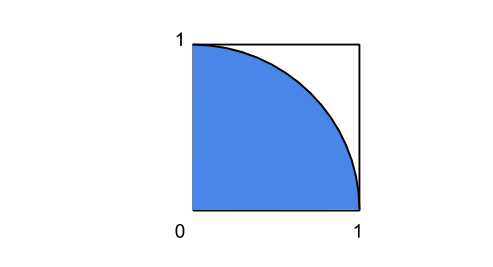
\includegraphics[width=\linewidth]{dartboard}
    \caption{The "dartboard." The computer throws a dart by choosing a random $x$ and $y$ between 0 and 1.  If $x^{2} + y^{2} < 1^{2} $, the dart landed inside the circle.  $A$ and $B$ are darts that landed inside the circle, while $C$ did not.}
    \label{dartboard}
\end{figure}

To stress test our framework, we ran a Monte-Carlo approximation of $\pi$. This process is largely analogous to having a square with the top-right quarter of a circle going through it (Fig. \ref{dartboard}), and then throwing darts at random locations.  Counting the ratio of darts that land inside the circle to the total number of throws gives us an approximation of $\frac{\pi}{4}$.  The more darts thrown, i.e. the more samples that are taken, the more accurate the approximation\footnote{This is not intended to be a particularly good approximation of $\pi$. Each additional digit of accuracy requires increasing the number of samples taken by an order of magnitude.}.

We chose this experiment for a number of reasons. The job is extremely easy to distribute.  This also made it very easy to test scalability. By doubling the amount of samples, we can double the amount of work each node gets.  We could also test the effectiveness of distributing the job among different numbers of workers.

Each Map job is defined by the number of throws the node must make and yields a result containing the total number of throws and the number of throws that landed inside the circular section.  Reducing these results is then a matter of adding the respective fields together. 

We ran our experiments using Amazons's Elastic Compute Cloud (EC2) service.  Amazon EC2 allows users to purchase an arbitrary amount of virtual machines by the hour. Each node was an individual EC2 small instance \cite{amazon-instances} with a preconfigured Ubuntu 12.04 image.  These instances were capable enough to provide constant computation, but still weak enough that they would be overwhelmed by traffic on occasions, creating a constant churn effect in the ring.  

Once started, nodes retrieve the latest version of the code and run it as a service, automatically joining the network.  We can choose any arbitrary node as the stager and tell it to run the MapReduce process. We found that the network was robust enough that we could take a node we wanted to be the stager out of the network, modify its MapReduce test code, have it rejoin the network, and then run the new code without any problems. Since only the stager has to know how to create the Map tasks, the other nodes do not have to be updated and execute the new tasks they are given.

We ran our experiments on groups of 1, 10, 20, 30, and 40 workers, which generated a $10^{8}$ sample set and a $10^{9}$ sample set.  Additionally, we gathered data on a $10^{7}$ sample set using 1, 5, 10, 20, 30 workers.  To test churn, we ran an experiment where each node had an equal chance of leaving and joining the network and varied the level of churn over multiple runs.  

We also utilized a subroutine we wrote called $plot$, which sends a message sequentially around the ring to establish how many members there are.  If $plot$ failed to return in under a second, the ring was experiencing structural instability.

\subsection{Results}

\begin{figure}
    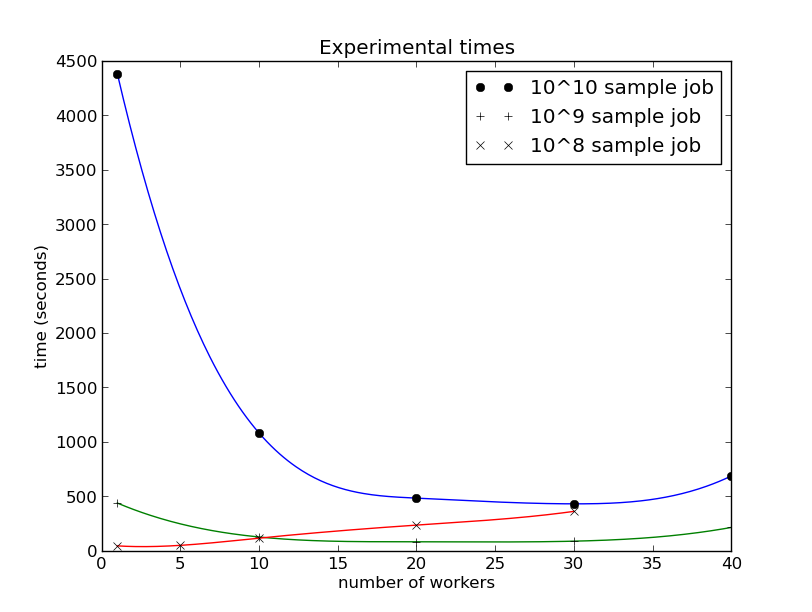
\includegraphics[width=\linewidth]{expTime}
    \caption{For a sufficiently large job, it was almost always preferable to distribute it.  When the job is too small, such as with the $10^{7}$ data set, our runtime is dominated by the overhead.  Our results are what we would expect when overhead grows logarithmically to the number of workers.}
    \label{expTime}
\end{figure}


\begin{figure}
    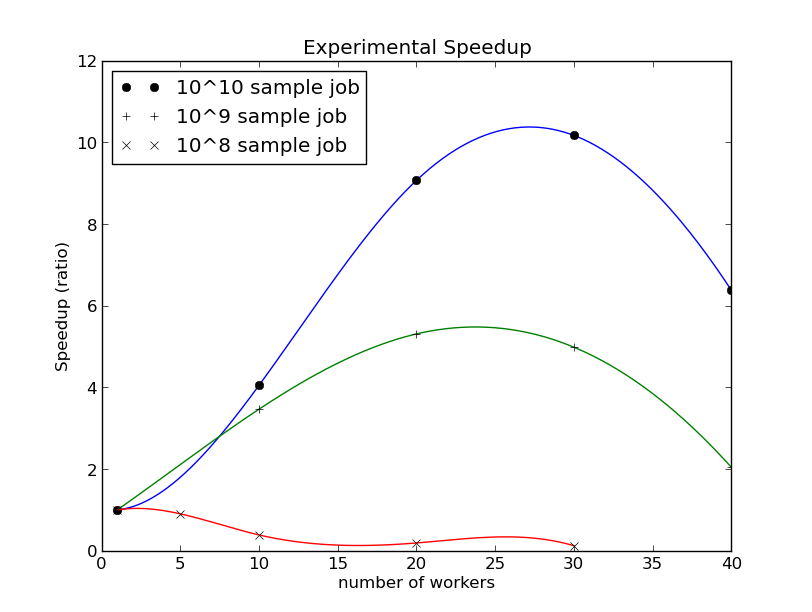
\includegraphics[width=\linewidth]{expSpeed}
    \caption{The larger the size of the job, the greater the gains of distributing with ChordReduce.  In addition, the larger the job, the more workers can be added before we start seeing diminishing returns.  This demonstrates that ChordReduce is scalable.}
    \label{expSpeed}
\end{figure}

Fig. \ref{expTime} and Fig. \ref{expSpeed} summarize the experimental results of job duration and speedup.  Our default series was the $10^{8}$ samples series.  On average, it took a single node 431 seconds, or approximately 7 minutes, to generate $10^{8}$ samples.  Generating the same number of samples using ChordReduce over 10, 20, 30, or 40 nodes was always quicker.  The samples were generated fastest when there were 20 workers, with a speedup factor of 4.96, while increasing the number of workers to 30 yielded a speedup of only 4.03.  At 30 nodes, the gains of distributing the work were present, but the cost of overhead ($k \cdot \log_{2}(n)$) had more of an impact.  This effect is more pronounced at 40 workers, with a speedup of 2.25.

Since our data showed that approximating $\pi$ on one node with $10^{8}$ samples took approximately 7 minutes, collecting $10^{9}$ samples on a single node would take 70 minutes at minimum.  Fig. \ref{expSpeed} shows that the $10^{9}$ set gained greater benefit from being distributed than the $10^{8}$ set, with the speedup factor at 20 workers being 9.07 compared to 4.03.  In addition, the gains of distributing work further increased at 30 workers and only began to decay at 40 workers, compared with the $10^{8}$ data set, which began its drop off at 30 workers. This behavior demonstrates that the larger the job being distributed, the greater the gains of distributing the work using ChordReduce.

The $10^{7}$ sample set confirms that the network overhead is logarithmic.  At that size, it is not effective to run the job concurrently and we start seeing overheard acting as the dominant factor in runtime.  This matches the behavior predicted by our equation, $T_{n} = \frac{T_{1}}{n} + k \cdot \log_{2}(n)$. For a small $T_{1}$, $\frac{T_{1}}{n}$  approaches 0 as $n$ gets larger, while $k \cdot \log_{2}(n)$, our overhead, dominates the sample.  The samples from our data set fit this behavior, establishing that our overhead increases logarithmically with the number of workers.


\begin{figure}
    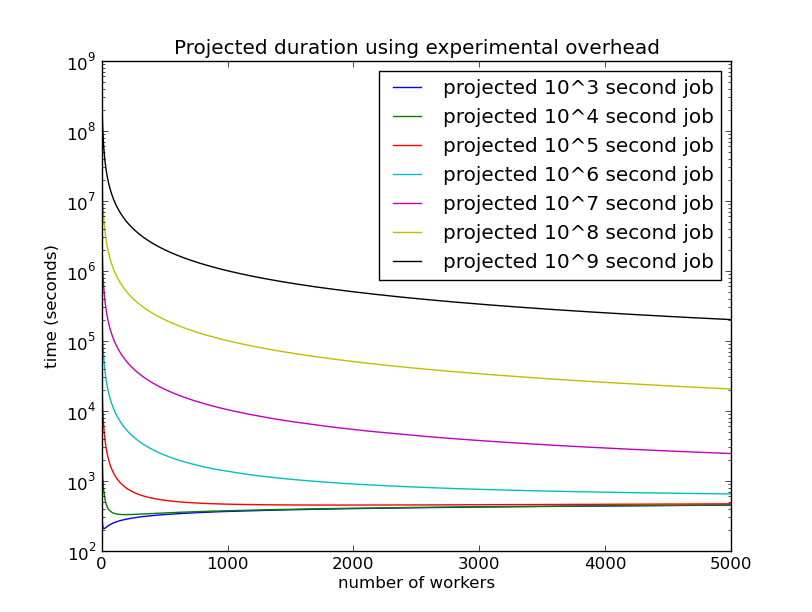
\includegraphics[width=\linewidth]{projTime}
    \caption{The projected runtime using ChordReduce for differently sized jobs.  Each curve projects the expected behavior for job that takes a single worker the specified amount of time.}
    \label{projTime}
\end{figure}

\begin{figure}
    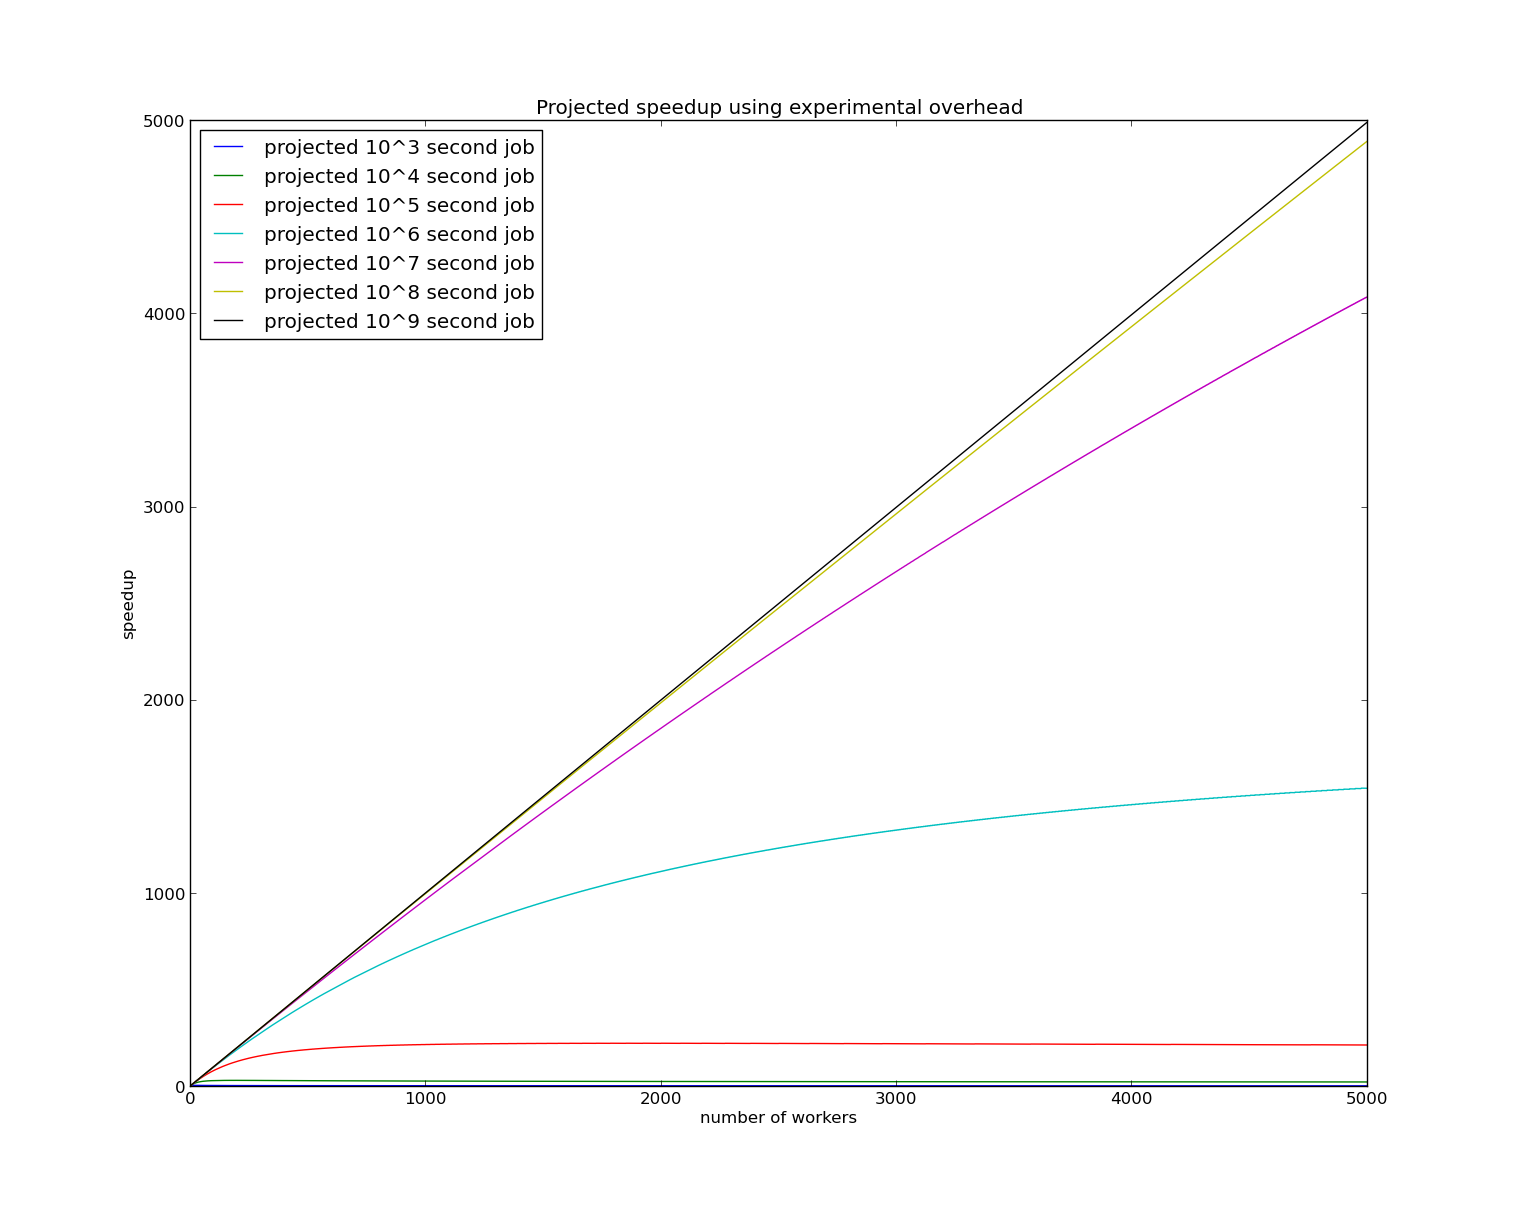
\includegraphics[width=\linewidth]{projSpeed}
    \caption{The projected speedup for different sized jobs. }
    \label{projSpeed}
\end{figure}

Since we have now established that $T_{n} = \frac{T_{1}}{n} + k \cdot \log_{2}(n)$, we can estimate how long a job that takes an arbitrary amount of time to run on a single node would take using ChordReduce.  Our data points indicated that the mean value of $k$ for this problem was 36.5.  Fig. \ref{projTime} shows that for jobs that would take more than $10^{4}$ seconds for single worker to complete, we can expect there would still be benefit to adding an additional worker, even when there are already 5000 workers already in the ring.  Fig. \ref{projSpeed} further emphasizes this. Note that as the jobs become larger, the expected speedup from ChordReduce  approaches linear behavior.


\begin{table}
    \centering
    \begin{tabular}{|r|r|r|} 
        \hline 
        Churn rate per second & Average runtime (s) & Speedup vs 0\% churn\\ \hline{}
        0.8\% & 191.25 & 2.15 \\ \hline
        0.4\% & 329.20 & 1.25 \\ \hline
        0.025\% & 431.86 & 0.95 \\ \hline 
        0.00775\%  & 445.47 & 0.92 \\ \hline 
        0.00250\% & 331.80  &  1.24 \\ \hline 
        0\% & 441.57 & 1.00 \\ \hline
    \end{tabular}
    \caption{} 
    \label{churnSpeed}
\end{table}


Table \ref{churnSpeed} shows the experimental results for different rates of churn. These results show the system  is relatively insensitive to churn.  We started with 40 nodes in the ring and generated $10^{8}$ samples while experiencing different rates of churn, as specified in Table \ref{churnSpeed}.  At the 0.8\% rate of churn, there is a 0.8\% chance each second that any given node will leave the network followed by another node joining the network at a different location. The joining rate and leaving rate being identical is not an unusual assumption to make \cite{marozzo2012p2p} \cite{load}.  

Our testing rates for churn are an order of magnitude higher than the rates used in the P2P-MapReduce simulation  \cite{marozzo2012p2p}.  In their paper, the highest rate of churn was only 0.4\% per minute. Because we were dealing with fewer nodes, we chose larger rates to demonstrate that ChordReduce could effectively handle a high level of churn.  


Our experiments show that for a given problem, ChordReduce can effectively distribute the problem, yielding a substantial speedup.  Furthermore, our results showed that the larger the problem is, the more workers could be added before diminishing returns were incurred.  During runtime, we experienced multiple instances where $plot$ would fail to run and the stager would report socket errors, indicating that it had lost connection with a node in the ring.  Despite this turbulence, every node managed to reestablish connection with each other and report back all the data.  This further demonstrated that we were able to handle the churn in the network.



\section{Related Work}

We have identified two papers that focus on combining P2P concepts with MapReduce.  Both papers are similar to our research, but differ in crucial ways, as described below.

%DEFINE ISSUES OF CHURN AND RELIABLILITY

\subsection{P2P-MapReduce}
Marozzo et al. \cite{marozzo2012p2p} investigated the issue of fault tolerance in centralized MapReduce architectures such as Hadoop.  They focused on creating a new P2P based MapReduce architecture built on JXTA \cite{935182} called P2P-MapReduce.  P2P-MapReduce is designed to be more robust at handling node and job failures during execution.

Rather than use a single master node, P2P-MapReduce employs multiple master nodes, each responsible for some job.  If one of those master nodes fails, another will be ready as a backup to take its place and manage the slave nodes assigned to that job.  This avoids the single point of failure that Hadoop is vulnerable to. Failures of the slave nodes are handled by the master node responsible for it.

Experimental results were gathered via simulation and compared P2P-MapReduce to a centralized framework. Their results showed that while P2P-MapReduce generated an order of magnitude more messages than a centralized approach, the difference rapidly began to shrink at higher rates of churn.  When looking at actual amounts of data being passed around the network, the bandwidth required by the centralized approach greatly increased as a function of churn, while the distributed approach again remained relatively static in terms of increased bandwidth usage.  

They concluded that P2P-MapReduce would, in general, use more network resources than a centralized approach. However, this was an acceptable cost as the P2P-MapReduce would lose less time from node and job failures \cite{marozzo2012p2p}.

While P2P-MapReduce is decentralized, it still relies on a very definite master/slave hierarchy for organization, computations, and scaling. 
During simulation, 1\% of the entire network was assigned as master nodes. This means for a simulation of 40000 nodes, 400 were required to organize and coordinate jobs, rendering them unable to do any processing.  In addition, a loosely-consistent  distributed hash table (DHT) such as JXTA can be much slower and fails to maintain the same level of guarantees as an actual DHT, such as Chord \cite{5359174}.   


%The loosely-consistent DHT can be much slower than using an acutal DHT such as Chord .
%Scalability.  A huge issue would be tracking all the nodes and coordinating them. Scalability is handled by mainataining a ratio of masters to slaves 
%Evaluated for low rates of churn.  Such low rates also mean master nodes are barely affected by churn.
%Simulations 
%Our work differs from Marozzo et al.'s in that P2P-MapReduce does not examine using the underlying strengths of a particular P2P protocol or group of protocols, which would have made the architecture simpler.  P2P-MapReduce is decentralized, but still relies on a very definite master/slave hierarchy, while all nodes in ChordReduce are both workers and masters.  We also implemented our MapReduce system rather than simulating the work.

\subsection{MapReduce using Symphony}

Lee et al.'s work \cite{leemap} draws attention to the fact that a P2P network can be much more than a way to distribute files and demonstrates how to accomplish different tasks using Map and Reduce functions over a P2P network.  Rather than using Chord, Lee et al. used Symphony \cite{symphony}, another DHT protocol with a ring topology.  To run a MapReduce job over the Symphony ring, a node is selected by the user to effectively act as the master.  This ad-hoc master then performs a bounded broadcast over a subsection the ring.  Each node repeats this broadcast over a subsection of that subsection, resulting in a tree with the first node at the top.  Map tasks are disseminated evenly throughout the tree and their results are reduced on the way back up to the ad-hoc master node.  This allows the ring to disseminate Map and Reduce tasks without the need for a coordinator responsible for distributing these tasks and keeping track of them, unlike Hadoop.
 
Their experimental results showed that the latency experienced by a centralized configuration is similar to the latency experienced in a completely distributed framework.  However, there are no mechanisms in place to handle churn in the network.  If a node joins during a MapReduce job, it will be unable to contribute any of its resources to the problem. If a node in the bounded broadcast tree fails, or worse the ad-hoc master node fails, the data that node is responsible for is lost. 

\section{Conclusion and Future Work}
We presented ChordReduce, a framework for MapReduce that is completely decentralized, scalable, load balancing, and highly tolerant to churn and node failure at any point in the network. We implemented a fully functional version of ChordReduce and performed detailed experiments to test its performance. These experiments confirmed that ChordReduce is robust and effective. ChordReduce is based on Chord, which is traditionally viewed as a P2P framework for distributing and sharing files.  Instead, we demonstrated that it can also be used as a platform for distributed computation.  Chord provides $\log_{2} n$ connectivity throughout network and has built in mechanisms for handling backup, automatically assigning responsibility, routing, and load balancing. 



Using Chord as the middleware for ChordReduce establishes its effectiveness for distributed and concurrent computation.
The effectiveness of Chord opens up new approaches for tackling other distributed problems, such as supporting databases and machine learning for Big Data, and exascale computations. We intend to further optimize the performance of ChordReduce and extend the middleware to other applications.




%For example, future work could incorporate processes that allow Chord to effectively share and distribute mutable files \cite{IRM} and alter them to perform distributed analysis of mutable data.  These same adjustments can be used to improve the latency of the Chord network with mutable data, which was a major reason why a Chord-based distributed DNS \cite{cox2002serving} was abandoned.  

%While ChordReduce is most efficient when each node is physically close in a cluster, minimizing the impact of latency, this does not exclude the option of tasks being distributed throughout the world.  This setup may be more applicable to a volunteer computing framework, such as Folding@home \cite{folding}.

%Many clusters assume identical or near identical hardware, running an equal amount of nodes, performing an equal amount of work. This is not always a safe assumption to make.  If the hardware used for computations is not equal, then some processors can be left idling when they could be doing more work, while others may be overwhelmed, holding back the rest of the network.

%Adjustments can be easily made on the user's end.  If some hardware can take more work than others, then that system can boot up more instances of nodes locally. Running two nodes locally would mean that approximately twice as much work would assigned to that computer.  Automatically balancing this load is also an avenue for future research.
%Chord could also be used to create a distributed authentication service.



%Our future plans for ChordReduce itself is to recode the library in Java to take advantage of the multiprocessing support, which is limited in Python. 

\section*{Appendix}

\lstinputlisting{pi.py}

\bibliographystyle{IEEEtran}
\bibliography{CHRONUS}
\end{document}

